% fig_vi_curves.tex
% IEC Very-Inverse (VI) time-current characteristic
% Three TMS values: fixed 0.12, adaptive 0.084, minimum clip 0.05
% Highlights HIF inverse-time operating window
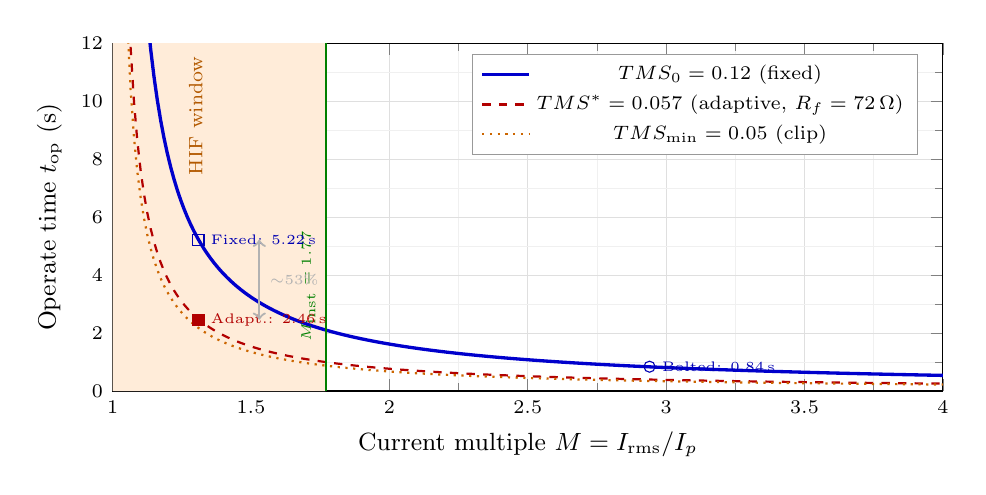
\begin{tikzpicture}
\begin{axis}[
  width=\columnwidth, height=6.0cm,
  xlabel={Current multiple $M = I_{\mathrm{rms}}/I_p$},
  ylabel={Operate time $t_{\mathrm{op}}$ (s)},
  xmin=1.0, xmax=4.0,
  ymin=0, ymax=12,
  xtick={1.0,1.5,2.0,2.5,3.0,3.5,4.0},
  ytick={0,2,4,6,8,10,12},
  minor tick num=1,
  grid=both,
  grid style={gray!25,line width=0.3pt},
  minor grid style={gray!12,line width=0.2pt},
  tick label style={font=\scriptsize},
  label style={font=\small},
  legend style={at={(0.97,0.97)},anchor=north east,
                font=\scriptsize,fill=white,draw=black!40},
  clip=true]

  % ---- HIF inverse-time window shading ----
  \addplot[fill=orange!15,draw=none,forget plot]
    coordinates {(1.0,0)(1.77,0)(1.77,12)(1.0,12)} \closedcycle;
  \node[font=\scriptsize,orange!70!black,align=center,rotate=90]
    at (axis cs:1.30,9.5) {HIF window};

  % ---- Fixed TMS = 0.12 ----
  \addplot[blue!80!black,very thick,samples=250,domain=1.005:4.0]
    { 0.12 * 13.5 / (x - 1.0) };
  \addlegendentry{$TMS_0 = 0.12$ (fixed)}

  % ---- Adaptive TMS = 0.057 (mid-HIF, Rf=72 ohm) ----
  \addplot[red!70!black,thick,dashed,samples=250,domain=1.005:4.0]
    { 0.057 * 13.5 / (x - 1.0) };
  \addlegendentry{$TMS^* = 0.057$ (adaptive, $R_f=72\,\Omega$)}

  % ---- Minimum TMS = 0.05 ----
  \addplot[orange!80!black,thick,dotted,samples=250,domain=1.005:4.0]
    { 0.05 * 13.5 / (x - 1.0) };
  \addlegendentry{$TMS_{\min} = 0.05$ (clip)}

  % ---- Instantaneous threshold ----
  \draw[green!50!black,thick]
    (axis cs:1.77,0) -- (axis cs:1.77,12)
    node[above,rotate=90,font=\tiny,green!50!black,pos=0.3]
    {$M_{\mathrm{inst}}=1.77$};

  % ---- Sample operating points ----
  % Bolted fault (M=2.94) — fixed
  \addplot[blue!70!black,only marks,mark=o,mark size=2pt,forget plot]
    coordinates {(2.94, 0.84)};
  \node[font=\tiny,blue!70!black,right=1pt]
    at (axis cs:2.94,0.84) {Bolted: 0.84\,s};

  % HIF (M=1.31) — fixed vs adaptive
  \addplot[blue!70!black,only marks,mark=square,mark size=2pt,forget plot]
    coordinates {(1.31, 5.22)};
  \node[font=\tiny,blue!70!black,right=1pt]
    at (axis cs:1.31,5.22) {Fixed: 5.22\,s};

  \addplot[red!70!black,only marks,mark=square*,mark size=2pt,forget plot]
    coordinates {(1.31, 2.46)};
  \node[font=\tiny,red!70!black,right=1pt]
    at (axis cs:1.31,2.46) {Adapt.: 2.46\,s};

  % ---- Delta-t annotation at M=1.31 ----
  \draw[<->,gray!60,thick]
    (axis cs:1.53,2.46) -- (axis cs:1.53,5.22)
    node[midway,right,font=\tiny,gray!60] {$\sim$53\%};

\end{axis}
\end{tikzpicture}
